\documentclass[letterpaper,10pt]{article}
% \usepackage{graphicx}
\usepackage{verbatim}
\usepackage{epsfig}

% \usepackage{}

\title{The MOOS-IvP Build System}
\author{Christian Convey (christian.convey@navy.mil)}
\date{2007-08-14}

\begin{document}

\maketitle

\begin{abstract}
This document details the design and intended use of MOOS-IvP's build system.
\end{abstract}

\tableofcontents

\parskip 7.2pt           % sets spacing between paragraphs

\section{HOWTO Build MOOS-IvP}
This section gives some basic background in using any CMake-based build system,
and then explains how to use MOOS-IvP's particular build system.

\subsection{CMake}

\subsubsection{Overview}
This section gives a brief overview of CMake, but clearer and more complete sources
of information exist:
\begin{itemize}
 \item The project's website: \verb|cmake.org|
 \item \underline{Mastering CMake}, by Ken Martin and Bill Hoffman.
 \item The CMake users email list: \verb|cmake@cmake.org|.  You can sign up
   for this at the \verb|cmake.org| website.
\end{itemize}


CMake (\verb|cmake.org|) is a cross-platform build system.  Compared to traditional 
Makefiles, CMake's control files (named \verb|CMakeLists.txt|) tend to be much shorter
and easier to read.

CMake has a number of back-ends for various operating systems and Make programs
(gmake, nmake, etc.) and IDEs (MS VisualStudio, KDevelop, Apple's XCode, etc.)
CMake-based build systems trivially support some features that can be a real
hassle to implement in hand-written Makefiles, such as calculating header file
dependencies and supporting an \verb|install| target.

The \verb|cmake| program reads in a project's \verb|CMakeLists.txt| files and produces
one or more files suitable for use in your build-system of choice (GNU Make, 
MS VisualStudio, etc.)  These generated build files will typically invoke the
\verb|cmake| program when building certain targets; therefore CMake must be installed
on any computer that will execute \verb|cmake|-produced build files.

\subsubsection{Language for Describing Makefiles}
\verb|CMakeLists.txt| files are written in an imperative language which is
documented on CMake's website.  The language lets you set variables and
supports branching, looping, and a limited form of subroutines (called
\verb|MACRO|'s).

When \verb|cmake| processes a project's \verb|CMakeLists.txt| files, the program
embodied in those files specifies the details of the build system to be created.
The \verb|CMakeLists.txt| files execute sequentially, specifying details as they
run.  Then end product is not a fully built version of your project, but rather
a set of build files (\verb|Makefile|, etc.) that when executed will build your
project.

The sequential nature of the programming language lets variables be computed,
helper programs run, conditions to be tested, etc. in order to determine what should
happen when the person building the project finally runs \verb|make| (or performs the
equivalent action in VisualStudio, XCode, etc. ).

\subsubsection{Federated Builds}
A typical CMake-based build system will contain one \verb|CMakeLists.txt| file
in each of the project's source tree's directories.  

The project's \textit{top-level} \verb|CMakeLists.txt| file typically sets variables that
govern the entire project's build details, such as the directory into which 
the built libraries and / or executables should be placed after being linked, and
the directory(ies) in which the project's header files can be found.

The \verb|CMakeLists.txt| files
in the \textit{internal levels} of the source tree often do nothing other than call
\verb|ADD_SUBDIRECTORY| on each of that directory's subdirectories.
(\verb|ADD_SUBDIRECTORY| is very
similar in effect to the C preprocessor's \verb|#include| directive.)
The practice of having intermediate-level directories' \verb|CMakeLists.txt|
files mostly just consist of \verb|ADD_SUBDIRECTORY| is common because
those directories often exist merely to group together 
subdirectories into units that are meaningful to the programmer.
Therefore those directories have little significance to the way the 
project code is actually built.

The source tree's \textit{leaf directories} typically contain the bulk of the project's 
interesting source code, with each subdirectory having the code for a single
library or executable.  The \verb|CMakeLists.txt| file in one of these leaf
directories will generally contain an \verb|ADD_LIBRARY| or \verb|ADD_EXECUTABLE|
command which leads to the compilation and linking of that one particular
program / library.

\subsubsection{Inherited Variables}
\verb|CMakeLists.txt| scripts have variables, similar in form and purpose
to \verb|make| shell variables.  They're treated and manipulated as text, and
lists are generally represented as a single string in which spaces separate
the list's elements.  (Another convention is sometimes used in CMake's functions,
where semicolons rather than spaces separate list elements.)

In traditional \verb|Makefile|s, a child \verb|make| process inherits a 
parent \verb|make| process' variable values.  A similar effect exists in
a hierarchy of \verb|CMakeLists.txt| files, but via a different mechanism:

Consider Figure \ref{fig:cmake-file-structure}.  Using these 
\verb|CMakeLists.txt| files would look like this:
\begin{verbatim}
cmake -f CMakeLists.txt
(... some miscellaneous output from cmake ...)
Y
X
(... some miscellaneous output from cmake ...)
\end{verbatim} 

Notice how the subdirectory's file \verb|Bar/CMakeLists.txt| not 
only inherits a value of \verb|MyVar| from the parent \verb|CMakeLists.txt| 
file, but \verb|Bar/CMakeLists.txt| also affects the behavior of the
parent \verb|CMakeLists.txt| file.  (\verb|Bar/CMakeLists.txt|) modifies
the value of \verb|MyVar|, and that new value is in effect in the 
lines of the parent \verb|CMakeLists.txt| file that follow the 
\verb|ADD_SUBDIRECTORY| call.  

Contrast this to behavior to a \verb|Makefile|-based system where 
a parent directory's \verb|Makefile| calls \verb|make -f Bar/Makefile|.
In that scenario, there is no mechanism by which \verb|Bar/Makefile|'s
modifications of \verb|make| variables could propagate back to the 
parent directory's running instance of \verb|make|.

\begin{figure}
 \centering
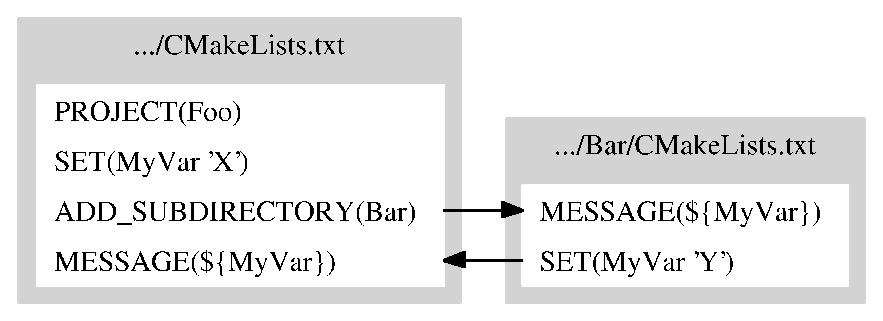
\includegraphics[width=4in]{file-structure.eps}
   \caption{ADD\_SUBDIRECTORY joines CMakeLists.txt files much like C's include}
   \label{fig:cmake-file-structure}
\end{figure}

\subsubsection{Cache Files}
Some CMake variables are computed each time you run \verb|cmake|, but other
\textit{cached} variables, once set, have their values recorded and stored in
a file named \verb|CMakeCache.txt|.  Variables stored in this file can be
edited using the \verb|ccmake| program (Linux) or the \verb|CMakeSetup.exe|
program (Windows).  This not only lets users enter certain data just one time
(i.e., the string that specifies the version of MOOS being built), but it also
exposes some CMake variables that whose value the user might want to correct.

For example, when CMake looks for the FLTK libraries, one variable that gets
set is \verb|FLTK_DIR|.  If CMake's \verb|FindFLTK| package can't figure out
where the FLTK libraries are, it will set the cached \verb|FLTK_DIR| variable
to have a value of \verb|FLTK_DIR-NOTFOUND|.  The user can run \verb|ccmake|
or \verb|CMakeSetup.exe| to manually set the value of \verb|FLTK_DIR| to
a valid value (typically \verb|/usr/lib| for that particular variable), and
then re-run \verb|cmake|.  This is typically enough of a help for a CMake
package such as \verb|FindFLTK| package to work out the rest of the details it
needs to.

Sometimes a \verb|CMakeCache.txt| file will contain so many bad values that
the user decides it's better just to start from scratch.  In general it's
safe for a user to manually delete a \verb|CMakeCache.txt| file.  When he
next runs \verb|cmake|, the variables whose values had been contained in the
file will simply be freshly computed.

\subsubsection{cmake, ccmake, CMakeSetup.exe}
\verb|cmake| is used to generate build-system files from a set of \verb|CMakeLists.txt|
files.  \verb|cmake| will also read from and write to a \verb|CMakeCache.txt| in the
directory from which \verb|cmake| is run.

Sometimes \verb|cmake| doesn't succeed the firs time it's run.  The FLTK module from
above is a good example.  We can easily write \verb|CMakeLists.txt| that would terminate
the \verb|cmake| invocation if the cached \verb|FLTK_DIR| variable had a value of \verb|FLTK_DIR-NOTFOUND|.

One solution to such a problem would be for the user to specify a good value on the
\verb|cmake| command line.  For example:
\begin{verbatim}
> cmake -DFLTK_DIR=/usr/lib -f CMakeLists.txt
\end{verbatim} 

This approach is sometimes the best, but \verb|ccmake| and \verb|CMakeSetup.exe| offer a
more interactive approach to configuring the build system.  Within these tools, you continue
re-running \verb|cmake| and modifing cached variable values until the \verb|cmake| succeeds.
At that point the user instructs the tool to ``generate'' the build system files (on Linux,
this typically includes a set of \verb|Makefile|s).  Once this is done the user will 
be ready to run \verb|make| (or whatever the equivalent action is for his build tool).

Note that \verb|ccmake| and \verb|CMakeSetup.exe| will not create the build system files
until the set of CMake variable values has stabilized.  This means that the tool must observe
that when it runs \verb|cmake|, none of the cached variables' values have changed.  This
relates to the fact that run \textit{n} of \verb|cmake| may set new value in a cached variable,
but the ramifications of that new variable aren't fully realized until the next invocation of
\verb|cmake| makes use of that value.

Practically speaking the need to iteratively run \verb|cmake| within \verb|ccmake| and \verb|CMakeSetup.exe| doesn't feel burdensome.  And if one knows the proper values for all
of the CMake variables of interest, you can set them on the \verb|cmake| command line 
as shown above, thus entirely avoiding the need to run \verb|ccmake| or
\verb|CMakeSetup.exe|.

\subsubsection{Finding External Packages}
\subsubsection{Configuring until Stable}
\subsubsection{In-source vs. Out-of-source Builds}

\subsection{Source Tree Organization and the Two Build Systems}

\subsection{Building MOOS-Ivp}
x

\subsection{Finding Needed Files}
x

\subsubsection{FLTK}
x

\subsubsection{Python.h}
x

\subsection{Other Important CMake Variables}
x
\subsection{Builds: In-source vs. Out-of-source}

\section{Implementation of MOOS-IvP Build System }
\subsection{Each Program / Library is Optional}
\subsection{Internal Dependencies}
- If building IvP on its own, then CMake sees things like MOOSGen as
a simple library dependency, so you must build MOOS first.
- If building MOOS-IvP as a combined project, CMake knows that MOOSGen
is another build target, and will understand dependencies.

\section{Future Work}


\subsection{Debian packaging}

\subsection{RPM packaging}

\subsection{Windows builds}

\subsection{Windows packaging}

\subsection{Building Documentation}

\subsection{Building IvP's Website}

\subsection{Supporing Release Creation}


\end{document}
